\documentclass[11pt]{article}
\usepackage[margin=0.75in]{geometry}
\usepackage{enumitem, amsmath, graphicx, booktabs}
\pagestyle{empty}

\title{A0 Poster Content\\{\large Future Alpha 2026}}
\author{Zaid Annigeri, MQF, Rutgers Business School}
\date{}
\begin{document}
\maketitle

\section*{TITLE}
Regime-Dependent Delta Hedging with SVI-Calibrated Volatility Surfaces on SPX Index Options

\section*{AUTHOR}
Zaid Annigeri | Master of Quantitative Finance | Rutgers Business School | ma.zaid@rutgers.edu

\section*{MOTIVATION}
Options desks choose their hedging volatility daily. The wrong choice generates unexplained P\&L variance that risk managers must reserve against and that erodes desk profitability. The Stochastic Volatility Inspired (SVI) parameterization is the industry standard for fitting implied volatility surfaces, yet no study has tested whether SVI-calibrated volatilities produce better delta-hedging outcomes than simpler alternatives. We conduct the first large-scale empirical comparison.

\section*{RESEARCH QUESTION}
Does SVI-calibrated surface volatility outperform flat BSM implied volatility and realized volatility estimators as a delta-hedging input? Is the optimal choice regime- and moneyness-dependent?

\section*{PRIOR WORK}
The Black-Scholes-Merton framework (Black and Scholes, 1973) assumes a single constant volatility for hedging, but implied volatility varies systematically across strikes and expirations. Gatheral's SVI parameterization (Gatheral, 2004; Gatheral and Jacquier, 2014) is the industry standard for fitting this surface, with typical RMSE of 10--50 bps. Hull and White (2017) showed that minimum-variance delta adjustments improve hedging by 2--10\% on SPX options, but did not test SVI. El Karoui et al.\ (1998) proved that BSM hedging is robust to volatility misspecification under domination conditions. \textbf{Gap:} No study has tested whether SVI-calibrated volatilities produce better hedging outcomes than flat IV or realized vol estimators. No study has decomposed hedging P\&L by VIX regime.

\section*{HYPOTHESES}
\begin{enumerate}[nosep]
\item[\textbf{H1:}] SVI surface vol reduces hedging error vs.\ flat BSM $\to$ \textbf{REJECTED} (Gain $= -9.4\%$, $p < 0.001$)
\item[\textbf{H2:}] Yang-Zhang RV outperforms Close-to-Close RV $\to$ \textbf{REJECTED} (CC wins by 24 percentage points)
\item[\textbf{H3:}] Optimal vol input is regime-dependent $\to$ \textbf{PARTIAL SUPPORT} (SVI wins OTM calls in Normal/High VIX; CC wins OTM puts across all regimes)
\end{enumerate}

\section*{DATA}
\begin{itemize}[nosep]
\item Source: OptionMetrics IvyDB US, SPX European options
\item Period: January 2019 -- December 2024
\item Scale: 28.6M raw observations $\to$ 5.6M filtered $\to$ 2{,}000 stratified sample
\item Stratification: 500 options per VIX regime (Low / Normal / High / Crisis)
\item Market events: COVID crash (VIX 82.7), 2022 rate hikes, 2023--24 normalization
\end{itemize}

\noindent\textbf{Figure --- SPX \& VIX with Regime Shading:}\\[0.5em]
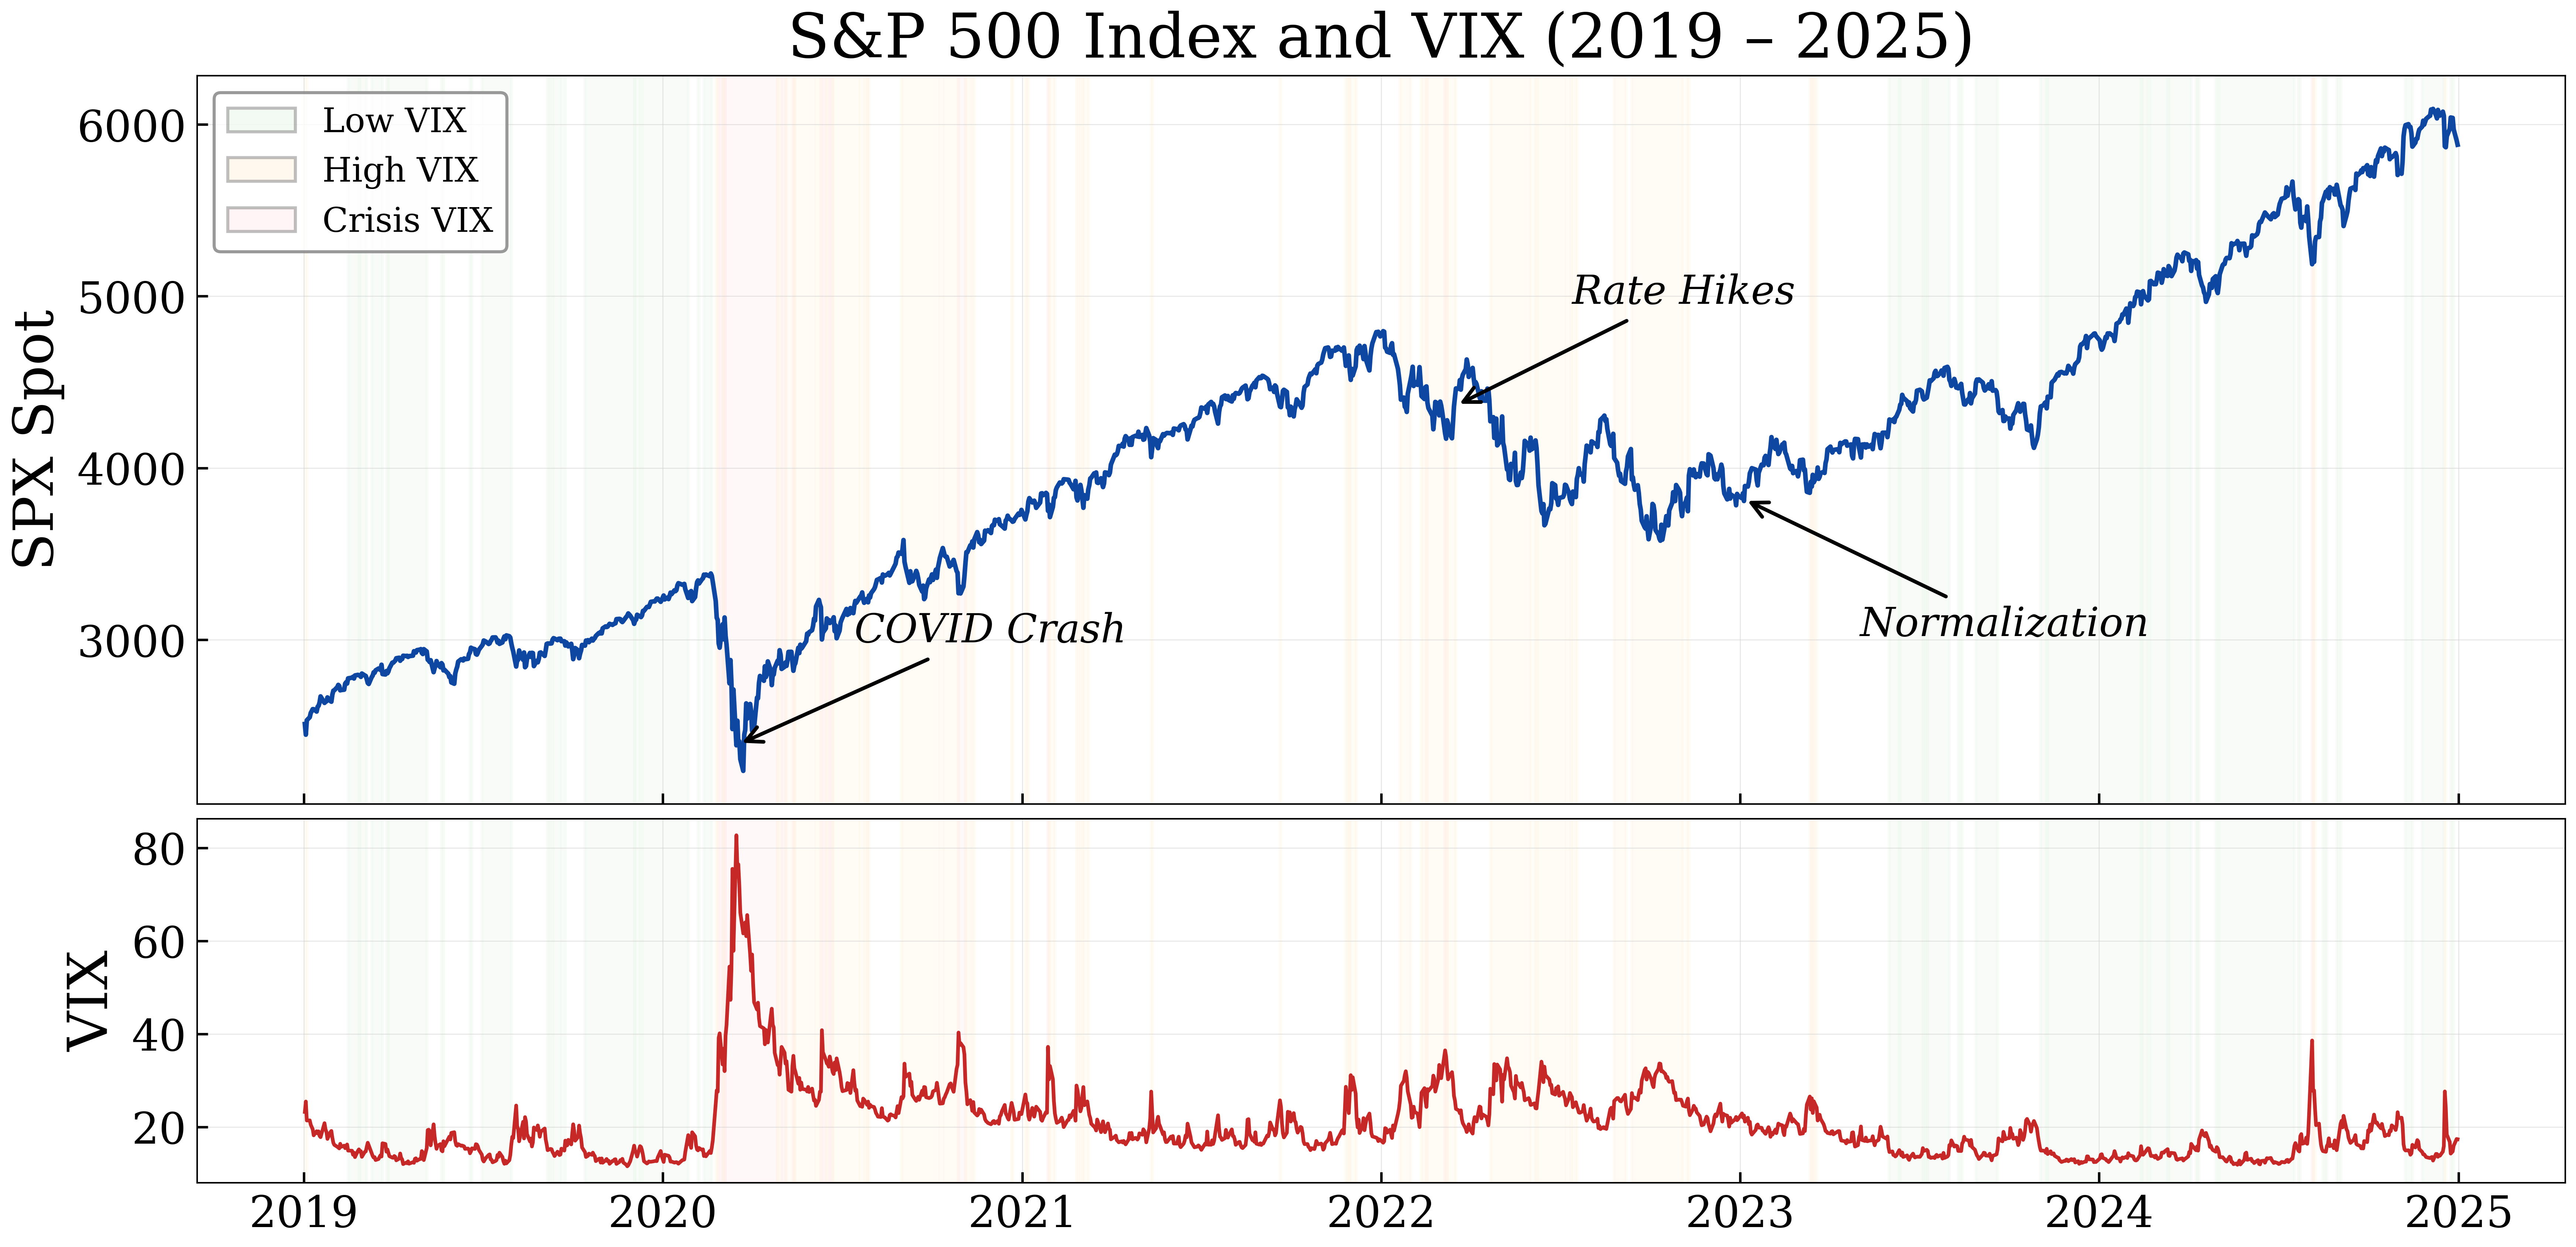
\includegraphics[width=\textwidth]{fig_poster_spx_vix.png}

\section*{SVI CALIBRATION OVER TIME}
\noindent\textbf{Figure --- SVI Calibration RMSE (bps) Time Series:}\\[0.5em]
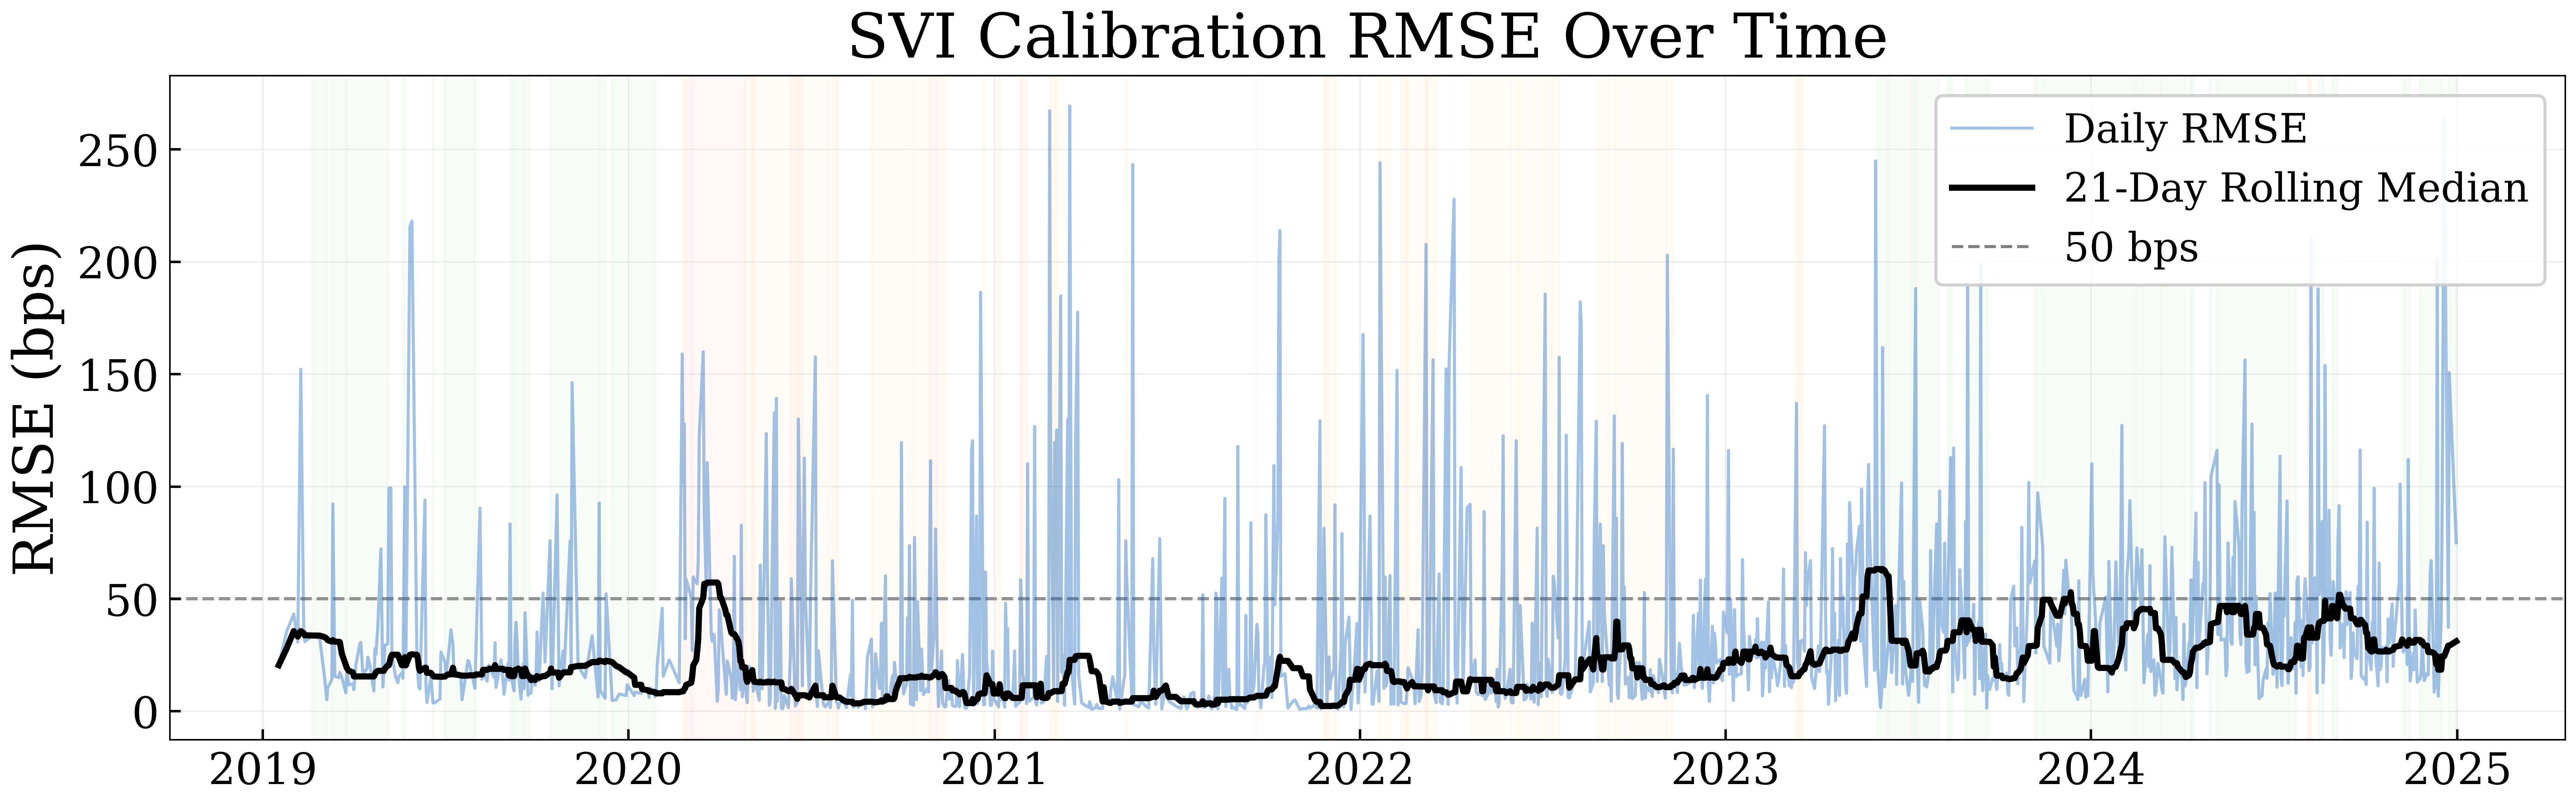
\includegraphics[width=\textwidth]{fig_poster_svi_rmse_timeseries.png}

\section*{METHODOLOGY}
\begin{itemize}[nosep]
\item \textbf{SVI Calibration:} Gatheral raw SVI parameterization $w(k) = a + b[\rho(k-m) + \sqrt{(k-m)^2 + \sigma^2}]$, 3-stage optimizer (LS $\to$ DE $\to$ L-BFGS-B), median RMSE 19.5 bps
\item \textbf{5 Volatility Inputs:} Flat BSM IV, SVI Surface IV, Close-to-Close RV, Parkinson RV, Yang-Zhang RV
\item \textbf{Hedging Protocol:} Sell option, BSM delta-hedge daily to expiry, measure hedging error
\item \textbf{4 VIX Regimes:} Low ($<$15), Normal (15--25), High (25--35), Crisis ($\geq$35)
\item \textbf{P\&L Decomposition:} El Karoui et al.\ (1998) framework --- discrete rebalancing + vol misspecification + higher-order residual
\item \textbf{Statistical Tests:} Paired $t$-tests, $F$-tests, Diebold-Mariano tests
\end{itemize}

\subsection*{Key Equations}
BSM Delta:
\begin{equation*}
\Delta_{\text{call}} = e^{-qT}\,\Phi(d_1), \quad d_1 = \frac{\ln(S/K) + (r - q + \tfrac{1}{2}\sigma^2)T}{\sigma\sqrt{T}}
\end{equation*}

SVI Total Implied Variance:
\begin{equation*}
w(k) = a + b\left[\rho(k - m) + \sqrt{(k-m)^2 + \sigma^2}\right], \quad k = \ln(K/F)
\end{equation*}

El Karoui P\&L Decomposition:
\begin{equation*}
\varepsilon_t = \underbrace{\tfrac{1}{2}\Gamma_t\left[(\Delta S_t)^2 - \sigma_h^2 S_t^2 \Delta t\right]}_{\text{Discrete Rebalancing}} + \underbrace{\tfrac{1}{2}\Gamma_t S_t^2(\sigma_r^2 - \sigma_h^2)\Delta t}_{\text{Vol Misspecification}} + \underbrace{\varepsilon_t^{\text{res}}}_{\text{Residual}}
\end{equation*}

\noindent\textbf{Figure --- SVI Fits by VIX Regime (2$\times$2 panel):}\\[0.5em]
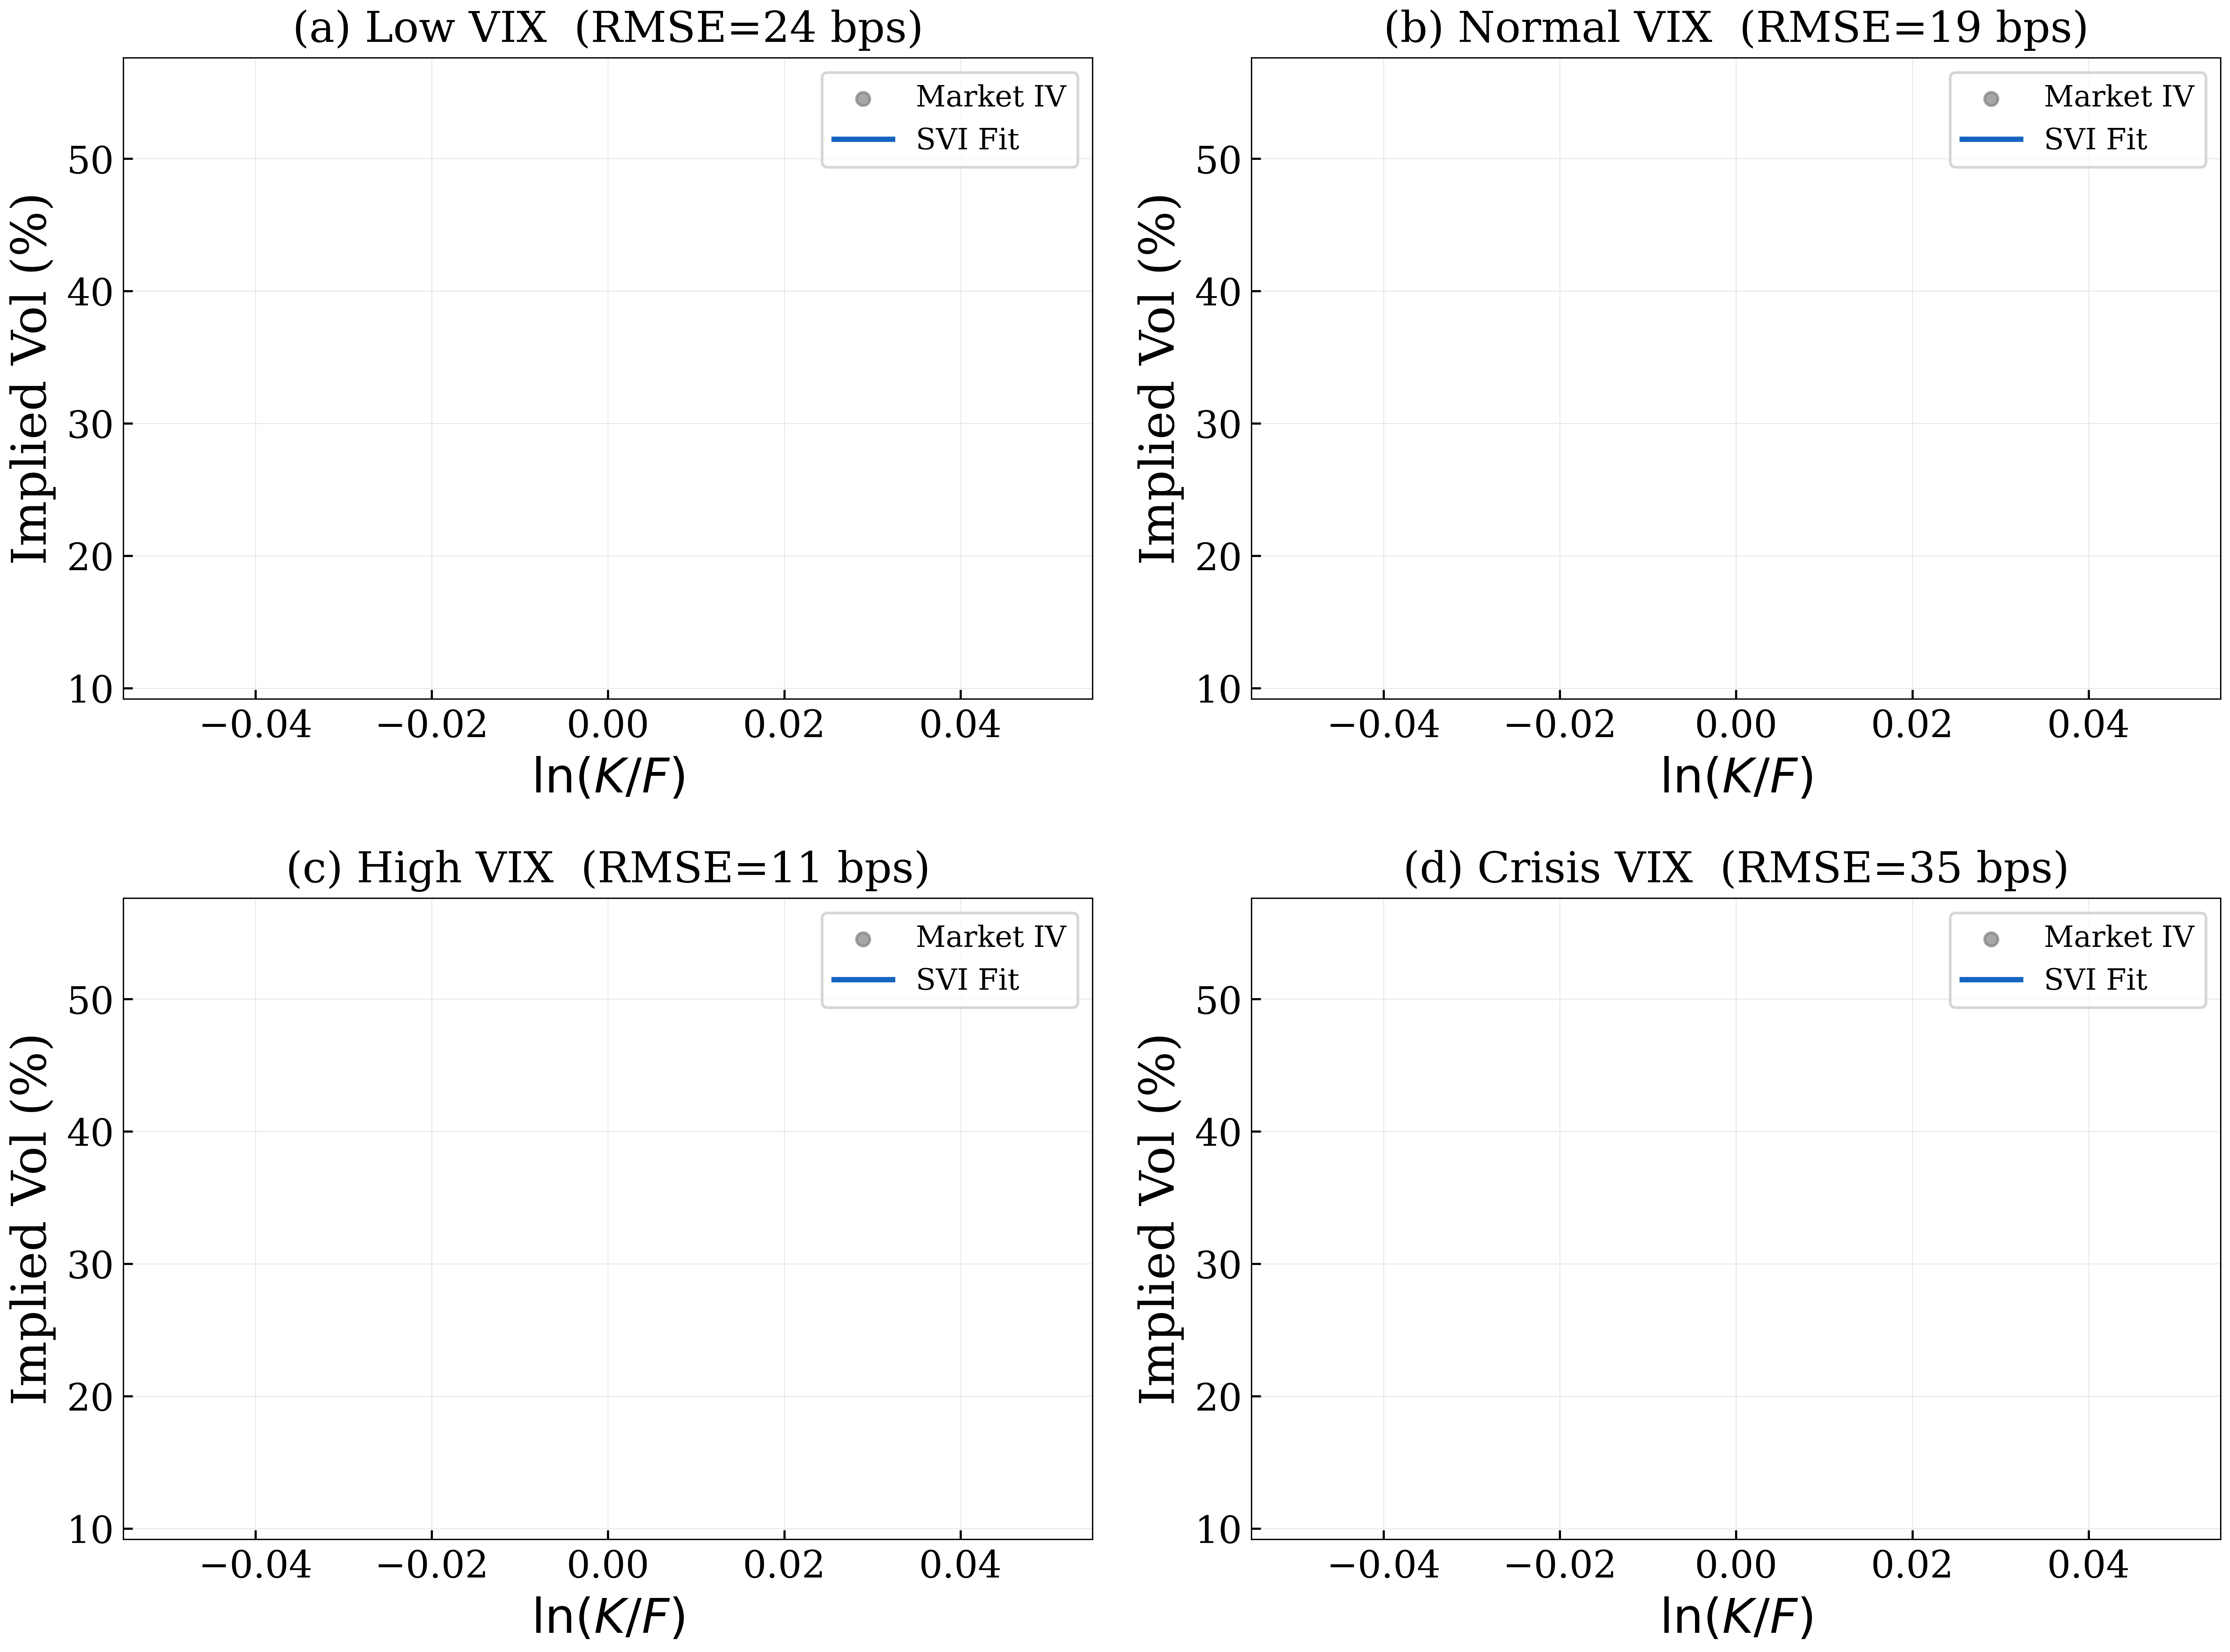
\includegraphics[width=\textwidth]{fig_poster_svi_fits.png}

\section*{VOLATILITY INPUTS EXPLAINED}
\begin{itemize}[nosep]
\item \textbf{Flat BSM IV:} ATM implied vol from OptionMetrics, constant across strikes for each expiry. Zero calibration error but ignores the smile.
\item \textbf{SVI Surface IV:} Strike-specific IV from calibrated Gatheral SVI surface. Captures smile shape but introduces 5-parameter estimation noise.
\item \textbf{Close-to-Close RV:} 21-day rolling standard deviation of log returns. Uses only closing prices. Simple but naturally aligned with how options reprice.
\item \textbf{Parkinson RV:} 21-day range-based estimator using daily high-low prices. 5$\times$ more efficient under GBM but sensitive to intraday noise.
\item \textbf{Yang-Zhang RV:} 21-day drift-independent OHLC estimator combining overnight, open-close, and range components. Most efficient theoretically but noisiest for hedging.
\end{itemize}

\section*{KEY RESULTS}
Close-to-close realized volatility achieves the best aggregate hedging performance, reducing hedging error standard deviation by 5.8\% versus the flat BSM benchmark ($F = 0.89$, $p = 0.008$). The SVI surface, despite achieving 19.5 basis points median calibration RMSE with 98\% convergence, increases hedging error variance by 9.4\% ($F = 1.20$, $p < 0.001$). However, the optimal input is strongly moneyness-dependent: SVI dominates for OTM calls (+6--12\% RMSE reduction), while close-to-close RV dominates for OTM puts (+21--48\% reduction). No single input wins everywhere.

\noindent\textbf{Figure --- Main Results Table:}\\[0.5em]
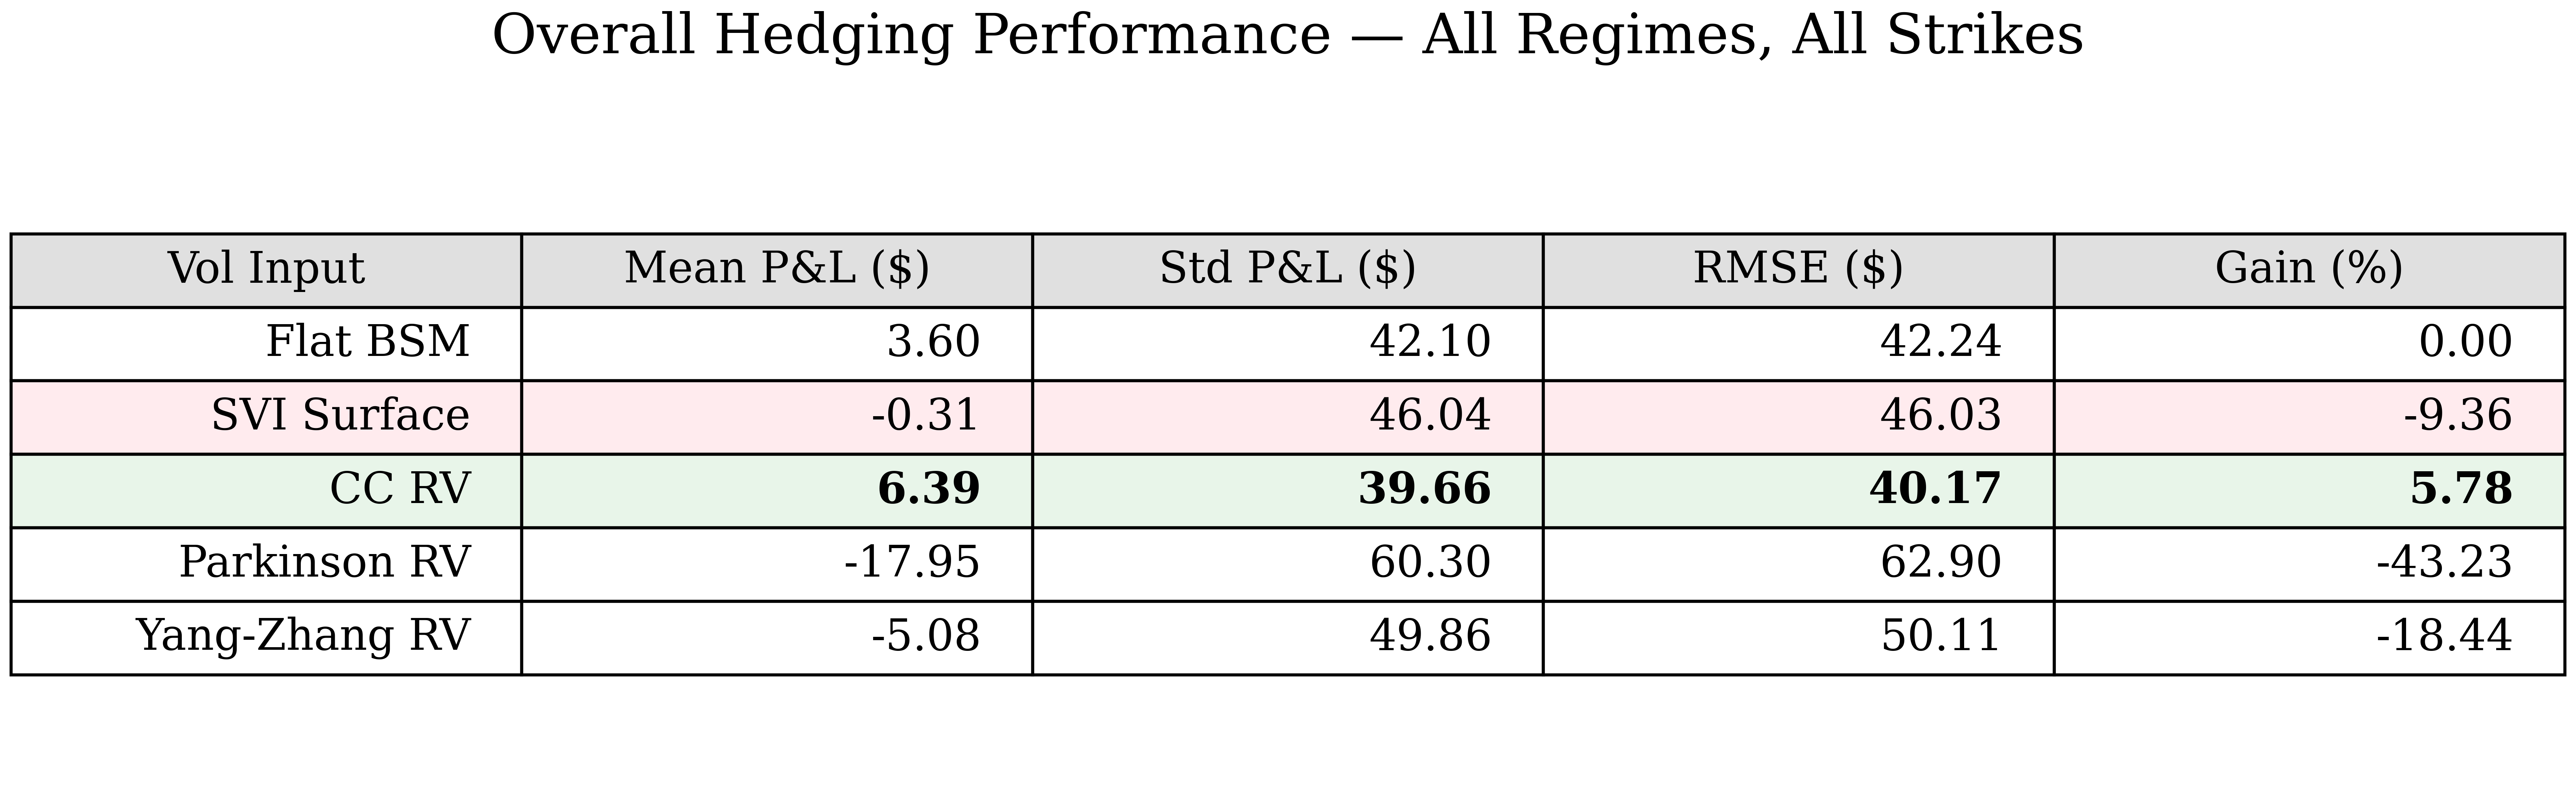
\includegraphics[width=\textwidth]{fig_poster_main_table.png}

\section*{REGIME-CONDITIONAL RESULTS}

\begin{tabular}{lcccc}
\hline
\textbf{Vol Input} & \textbf{Low} & \textbf{Normal} & \textbf{High} & \textbf{Crisis} \\
\hline
Flat BSM (Std \$) & 18.36 & 18.20 & 20.64 & 64.42 \\
SVI Surface (Gain\%) & $-$8.8\% & +0.8\% & +3.7\% & $-$2.3\% \\
CC RV (Gain\%) & $-$7.1\% & $-$15.3\% & $-$12.4\% & $-$4.0\% \\
\hline
\end{tabular}\\[0.5em]
SVI shows its only positive Gains in Normal (+0.8\%) and High (+3.7\%) VIX regimes, where the smile is steep enough to carry information but stable enough for reliable calibration. In Low and Crisis regimes, all alternatives add noise relative to flat BSM.

\section*{FINDING 1}
\textbf{More information $\neq$ better hedging.} SVI surface volatility increases hedging error by 9.4\% despite achieving 19.5 bps calibration RMSE. Calibration noise in the five-parameter optimization outweighs the informational benefit of strike-specific volatilities.

\noindent\textbf{Figure --- Hedging Error Std by VIX Regime:}\\[0.5em]
\includegraphics[width=\textwidth]{fig_poster_regime_bars.png}

\section*{FINDING 2}
\textbf{Simple wins.} Close-to-close realized volatility reduces hedging error by 5.8\% ($F = 0.89$, $p = 0.008$). The simplest estimator --- using only closing prices --- beats the most sophisticated alternatives that incorporate intraday price information.

\section*{FINDING 3}
\textbf{The answer is moneyness-dependent.} SVI wins for OTM calls (+6--12\% RMSE reduction), where the smile slope is steepest. RV wins for OTM puts (+21--48\%). No single volatility input dominates everywhere, motivating a conditional hedging strategy.

\noindent\textbf{Figure --- Best Vol Input by Moneyness $\times$ DTE:}\\[0.5em]
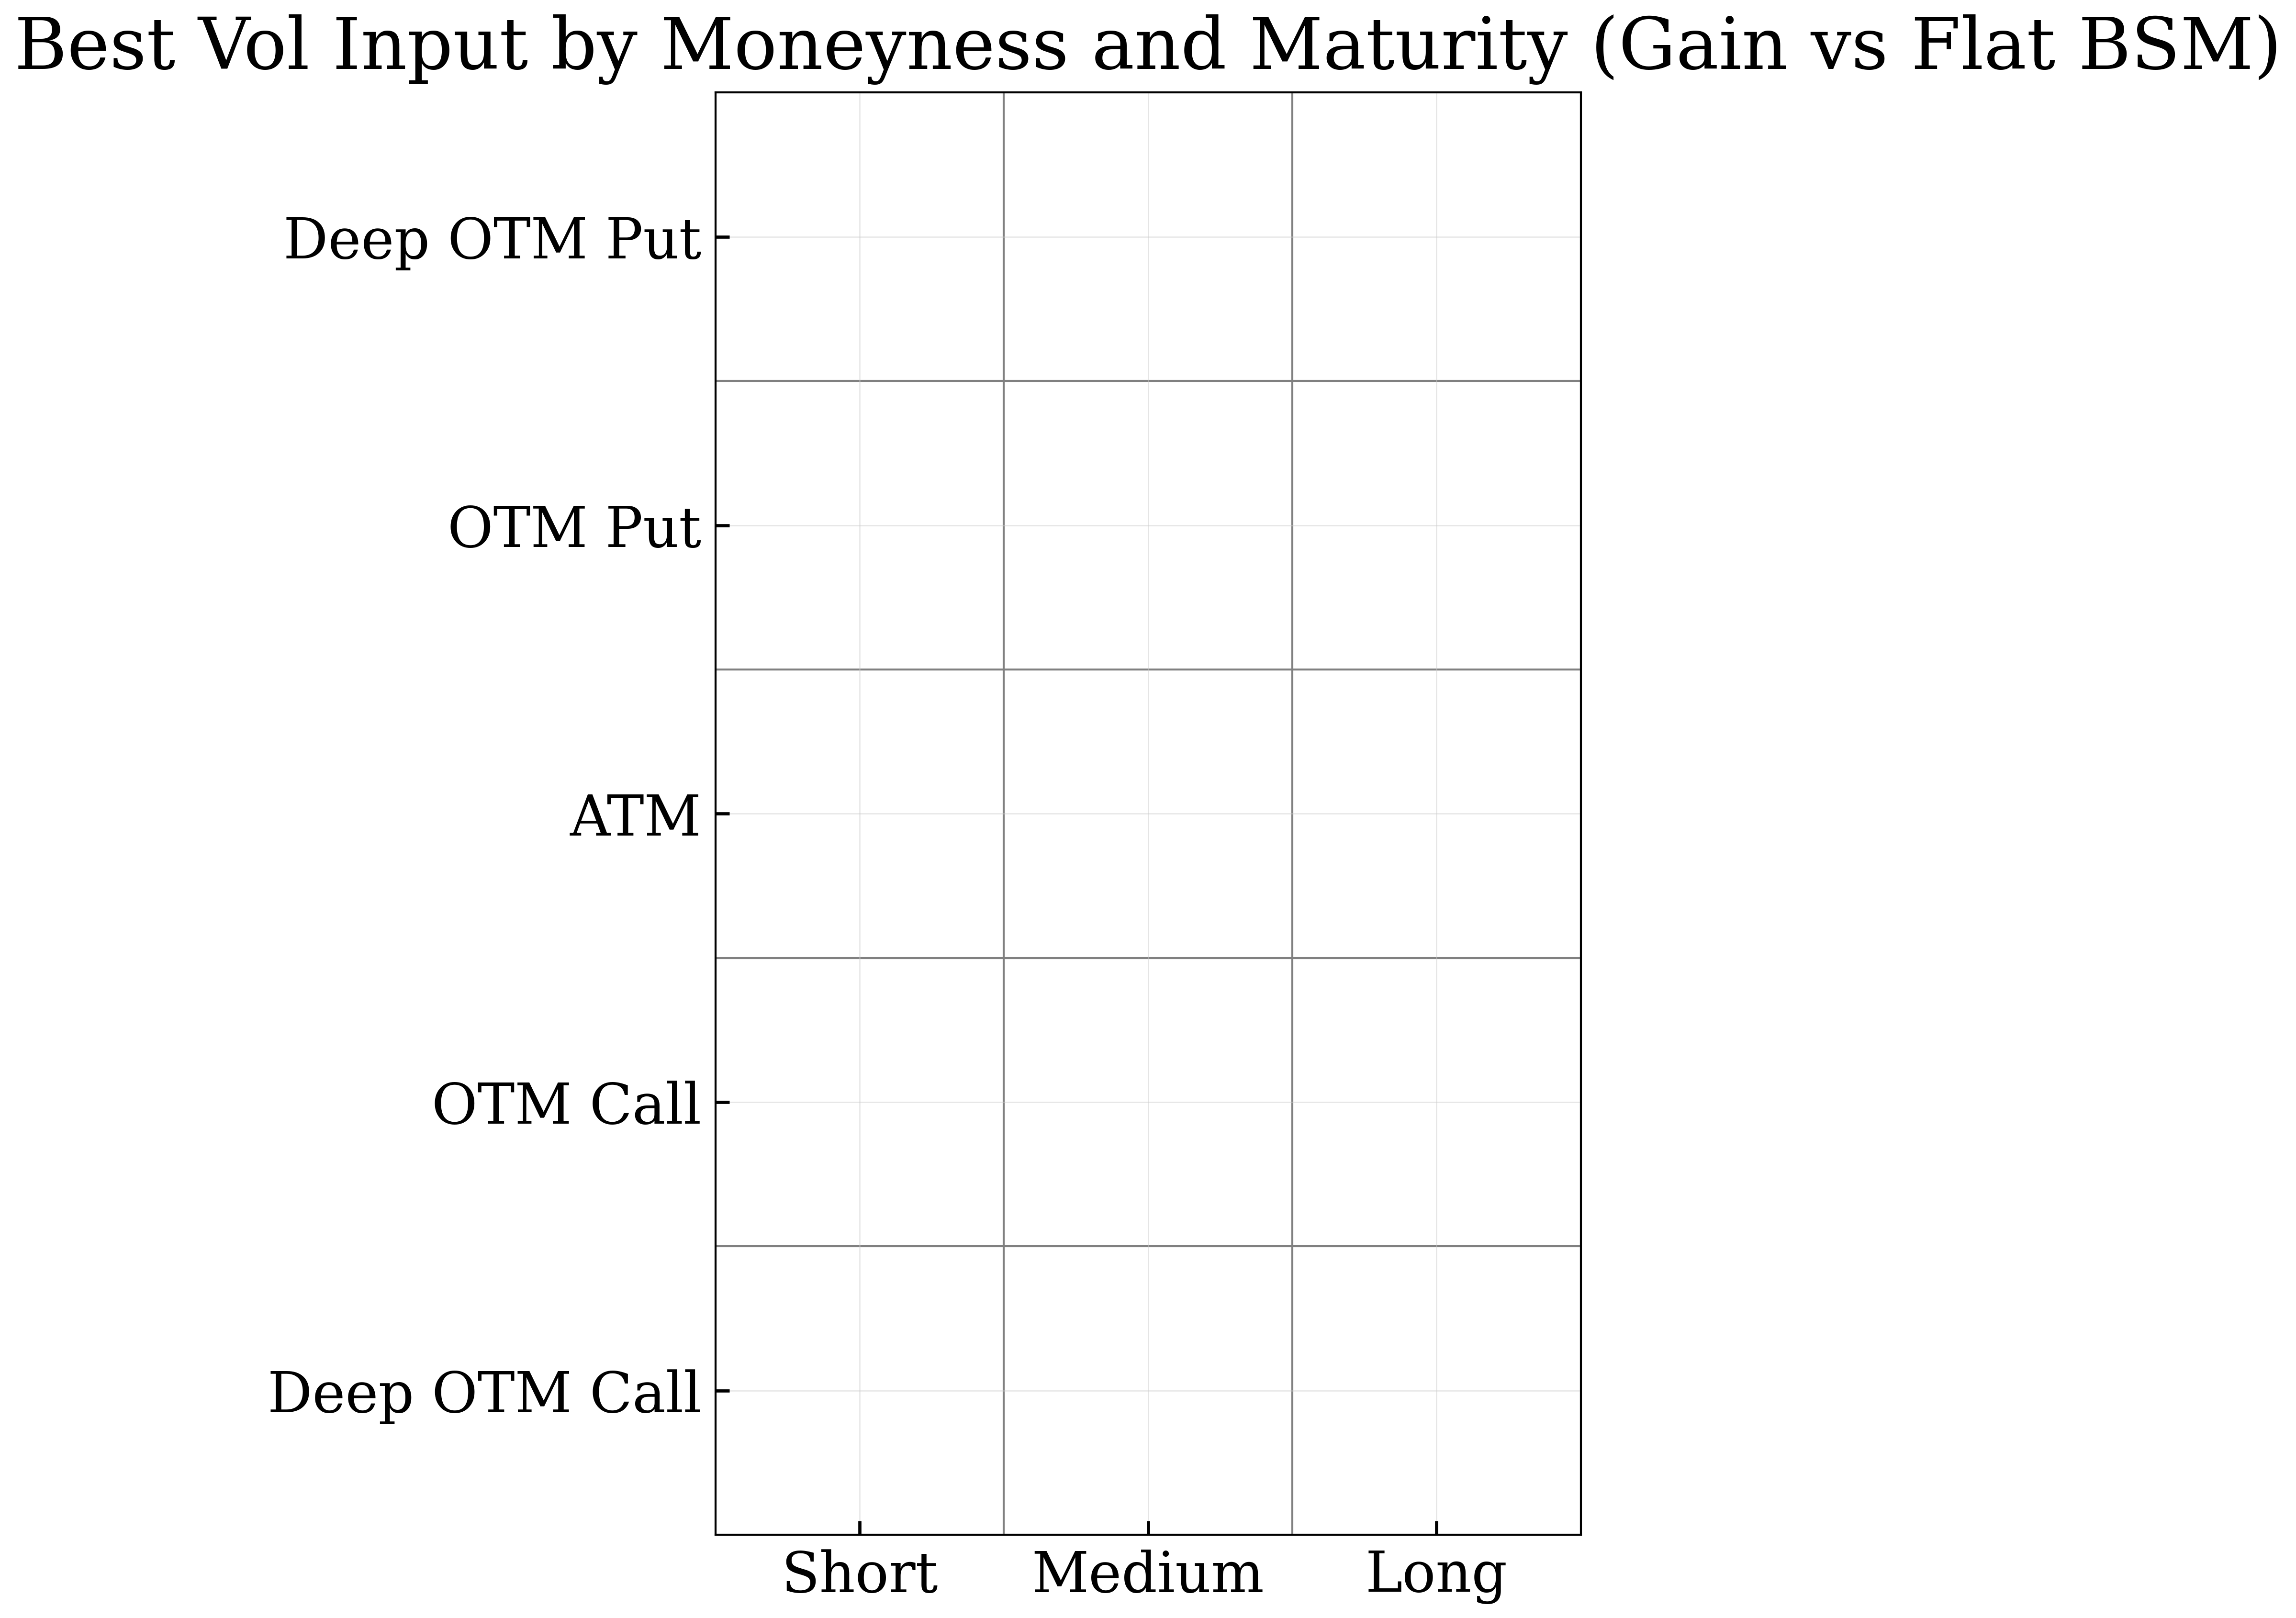
\includegraphics[width=\textwidth]{fig_poster_moneyness_grid.png}

\section*{REALIZED VS IMPLIED VOLATILITY}
\noindent\textbf{Figure --- Three RV Estimators vs ATM Implied Vol:}\\[0.5em]
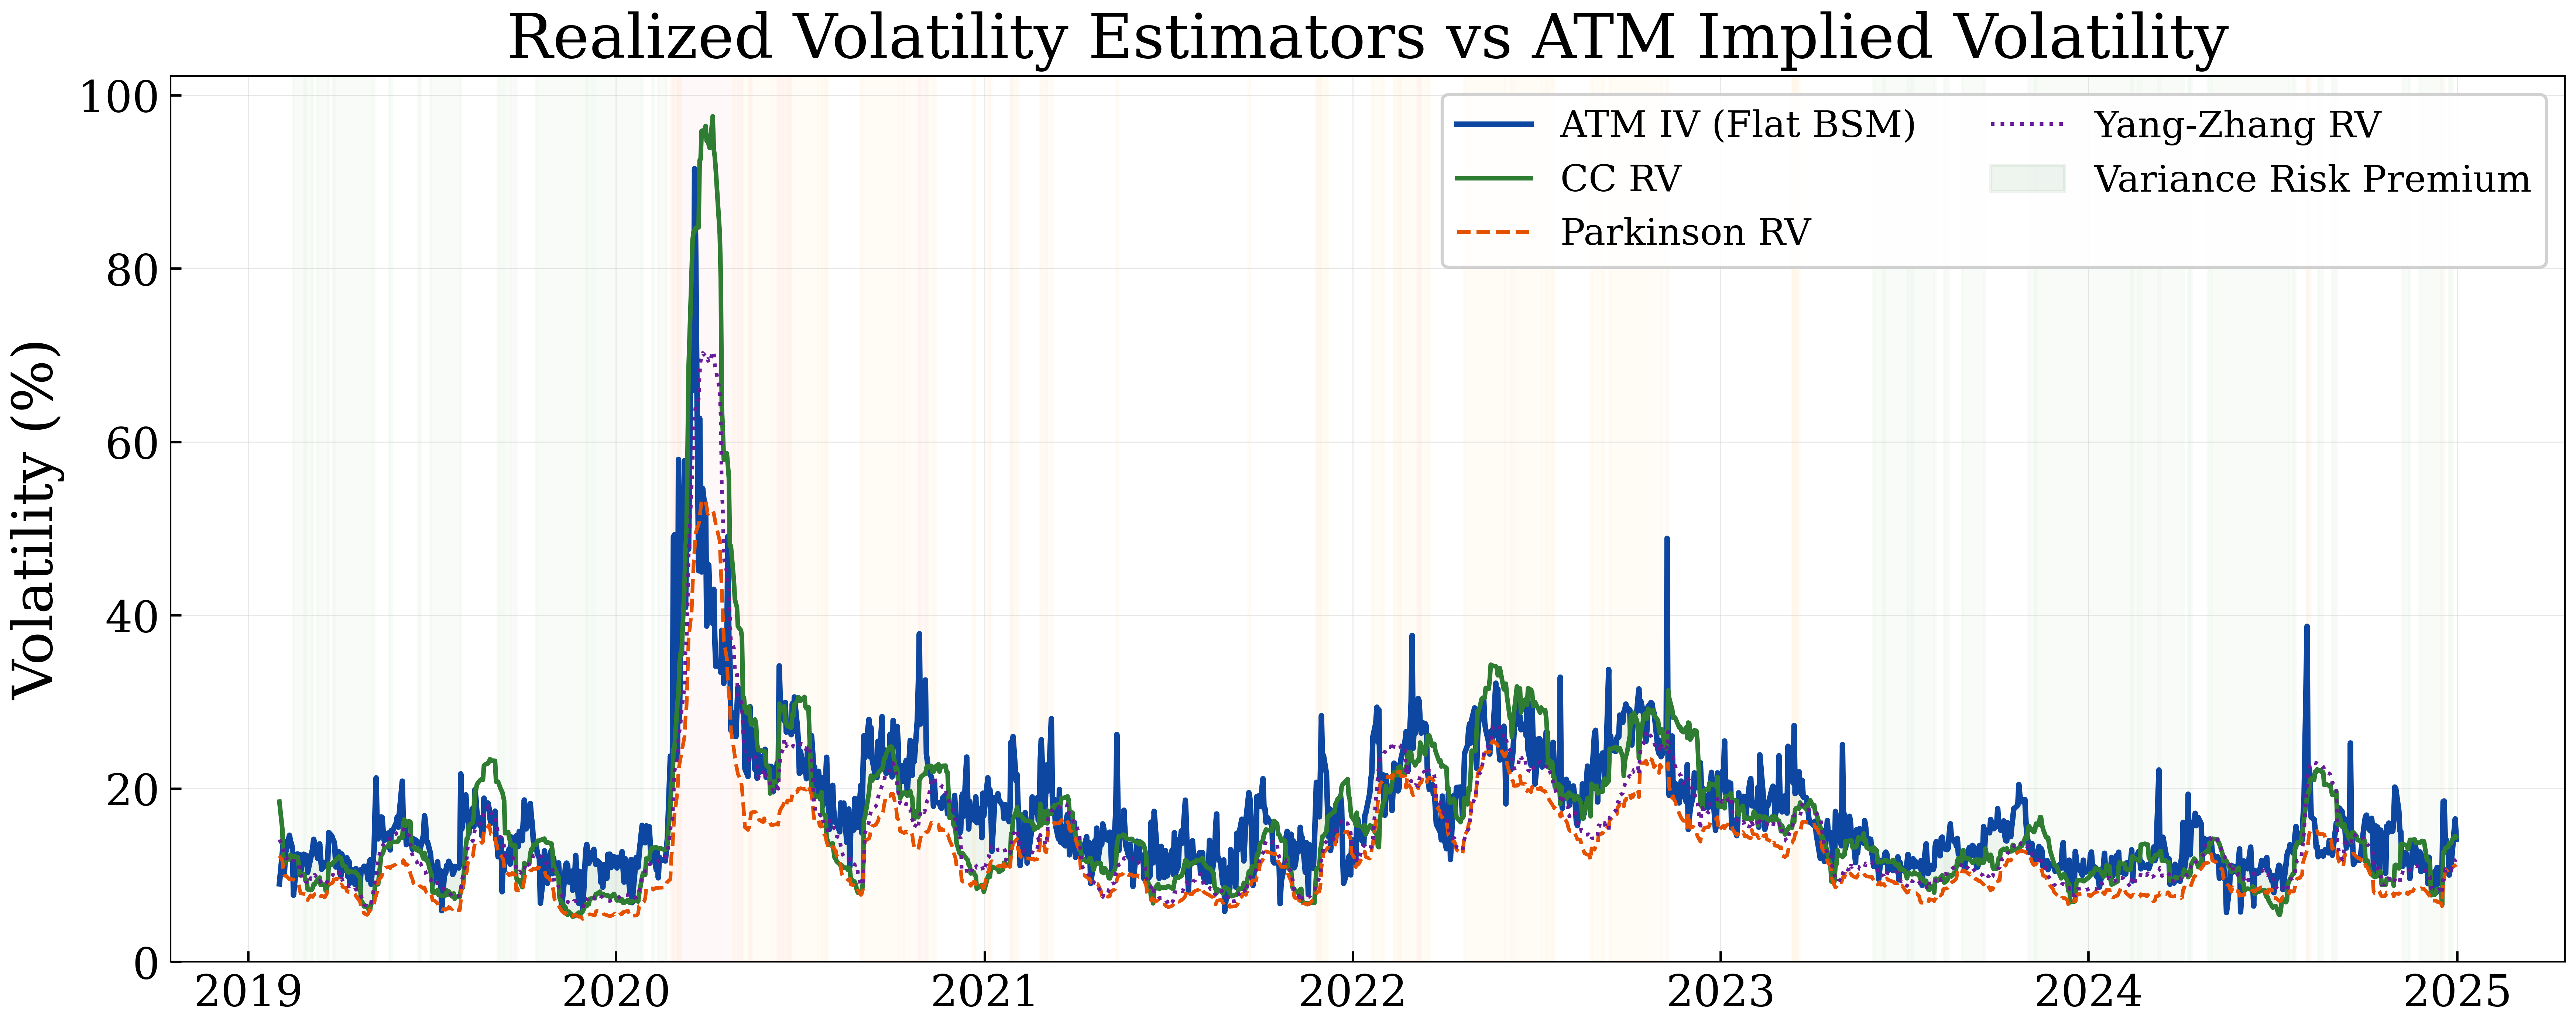
\includegraphics[width=\textwidth]{fig_poster_rv_vs_iv.png}

\section*{P\&L ATTRIBUTION}
We decompose hedging P\&L using the El Karoui et al.\ (1998) covariance-based framework. The results reveal that higher-order residual terms---capturing vanna (sensitivity of delta to vol), volga (sensitivity of vega to vol), jump risk, and discrete-time approximation error---account for 150--210\% of total hedging error variance across all four regimes. Discrete rebalancing error and vol misspecification are \textit{negatively} correlated with total P\&L, partially offsetting the residual. This implies that gamma management---reducing net gamma exposure---is more impactful than volatility input selection for controlling hedging error.

\noindent\textbf{Figure --- Covariance-Based P\&L Attribution:}\\[0.5em]
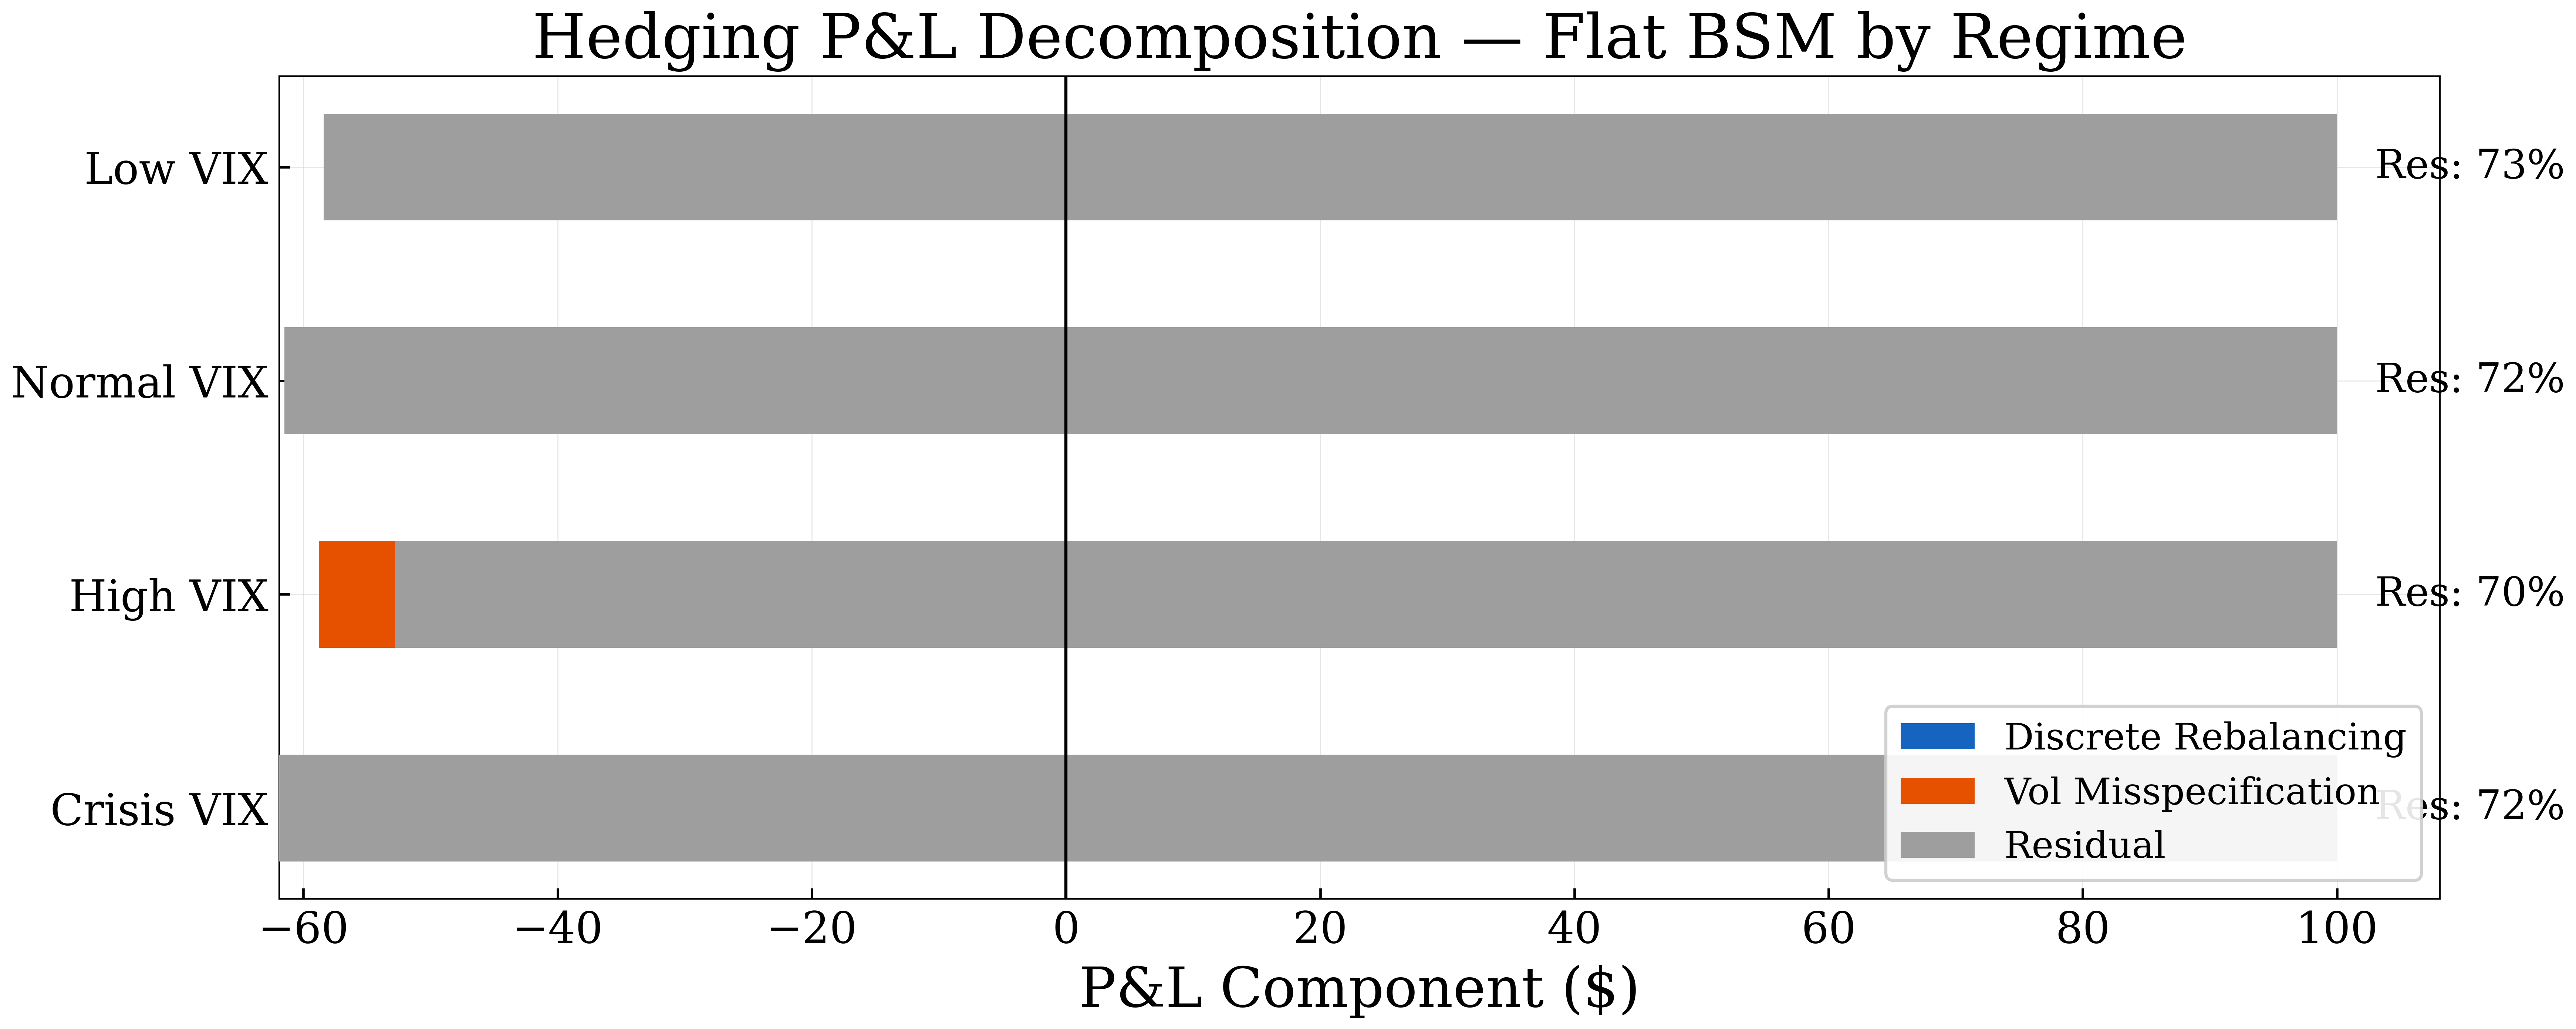
\includegraphics[width=\textwidth]{fig_poster_pnl_attribution.png}

\section*{WHY DOES THE SMILE HURT?}
Three mechanisms explain SVI's aggregate underperformance:
\begin{enumerate}[nosep]
\item \textbf{Calibration noise.} Every 5-parameter SVI optimization introduces estimation error that propagates into the hedge delta through $d_1$. Flat ATM IV uses a single observed price with zero calibration error.
\item \textbf{Interpolation artifacts.} Calibrating every 5th trading day and interpolating between dates introduces stale smile information. The hedge delta responds to yesterday's smile, not today's.
\item \textbf{Signal vs.\ noise tradeoff.} For OTM calls, the smile slope is steep and carries genuine hedgeable information (Gain +6--12\%). For ATM and OTM puts, the noise outweighs the signal.
\end{enumerate}

\section*{PRACTITIONER IMPLICATIONS}
Evidence-based hedging volatility selection:
\begin{itemize}[nosep]
\item OTM Call book $\to$ SVI Surface IV
\item OTM Put book $\to$ Close-to-Close Realized Vol
\item ATM book $\to$ Flat BSM IV
\item Crisis regime (VIX $\geq$ 35) $\to$ Focus on gamma management, not volatility input choice
\end{itemize}
A moneyness-conditional strategy outperforms any single-input approach.

\noindent\textbf{Figure --- Practitioner Decision Flowchart:}\\[0.5em]
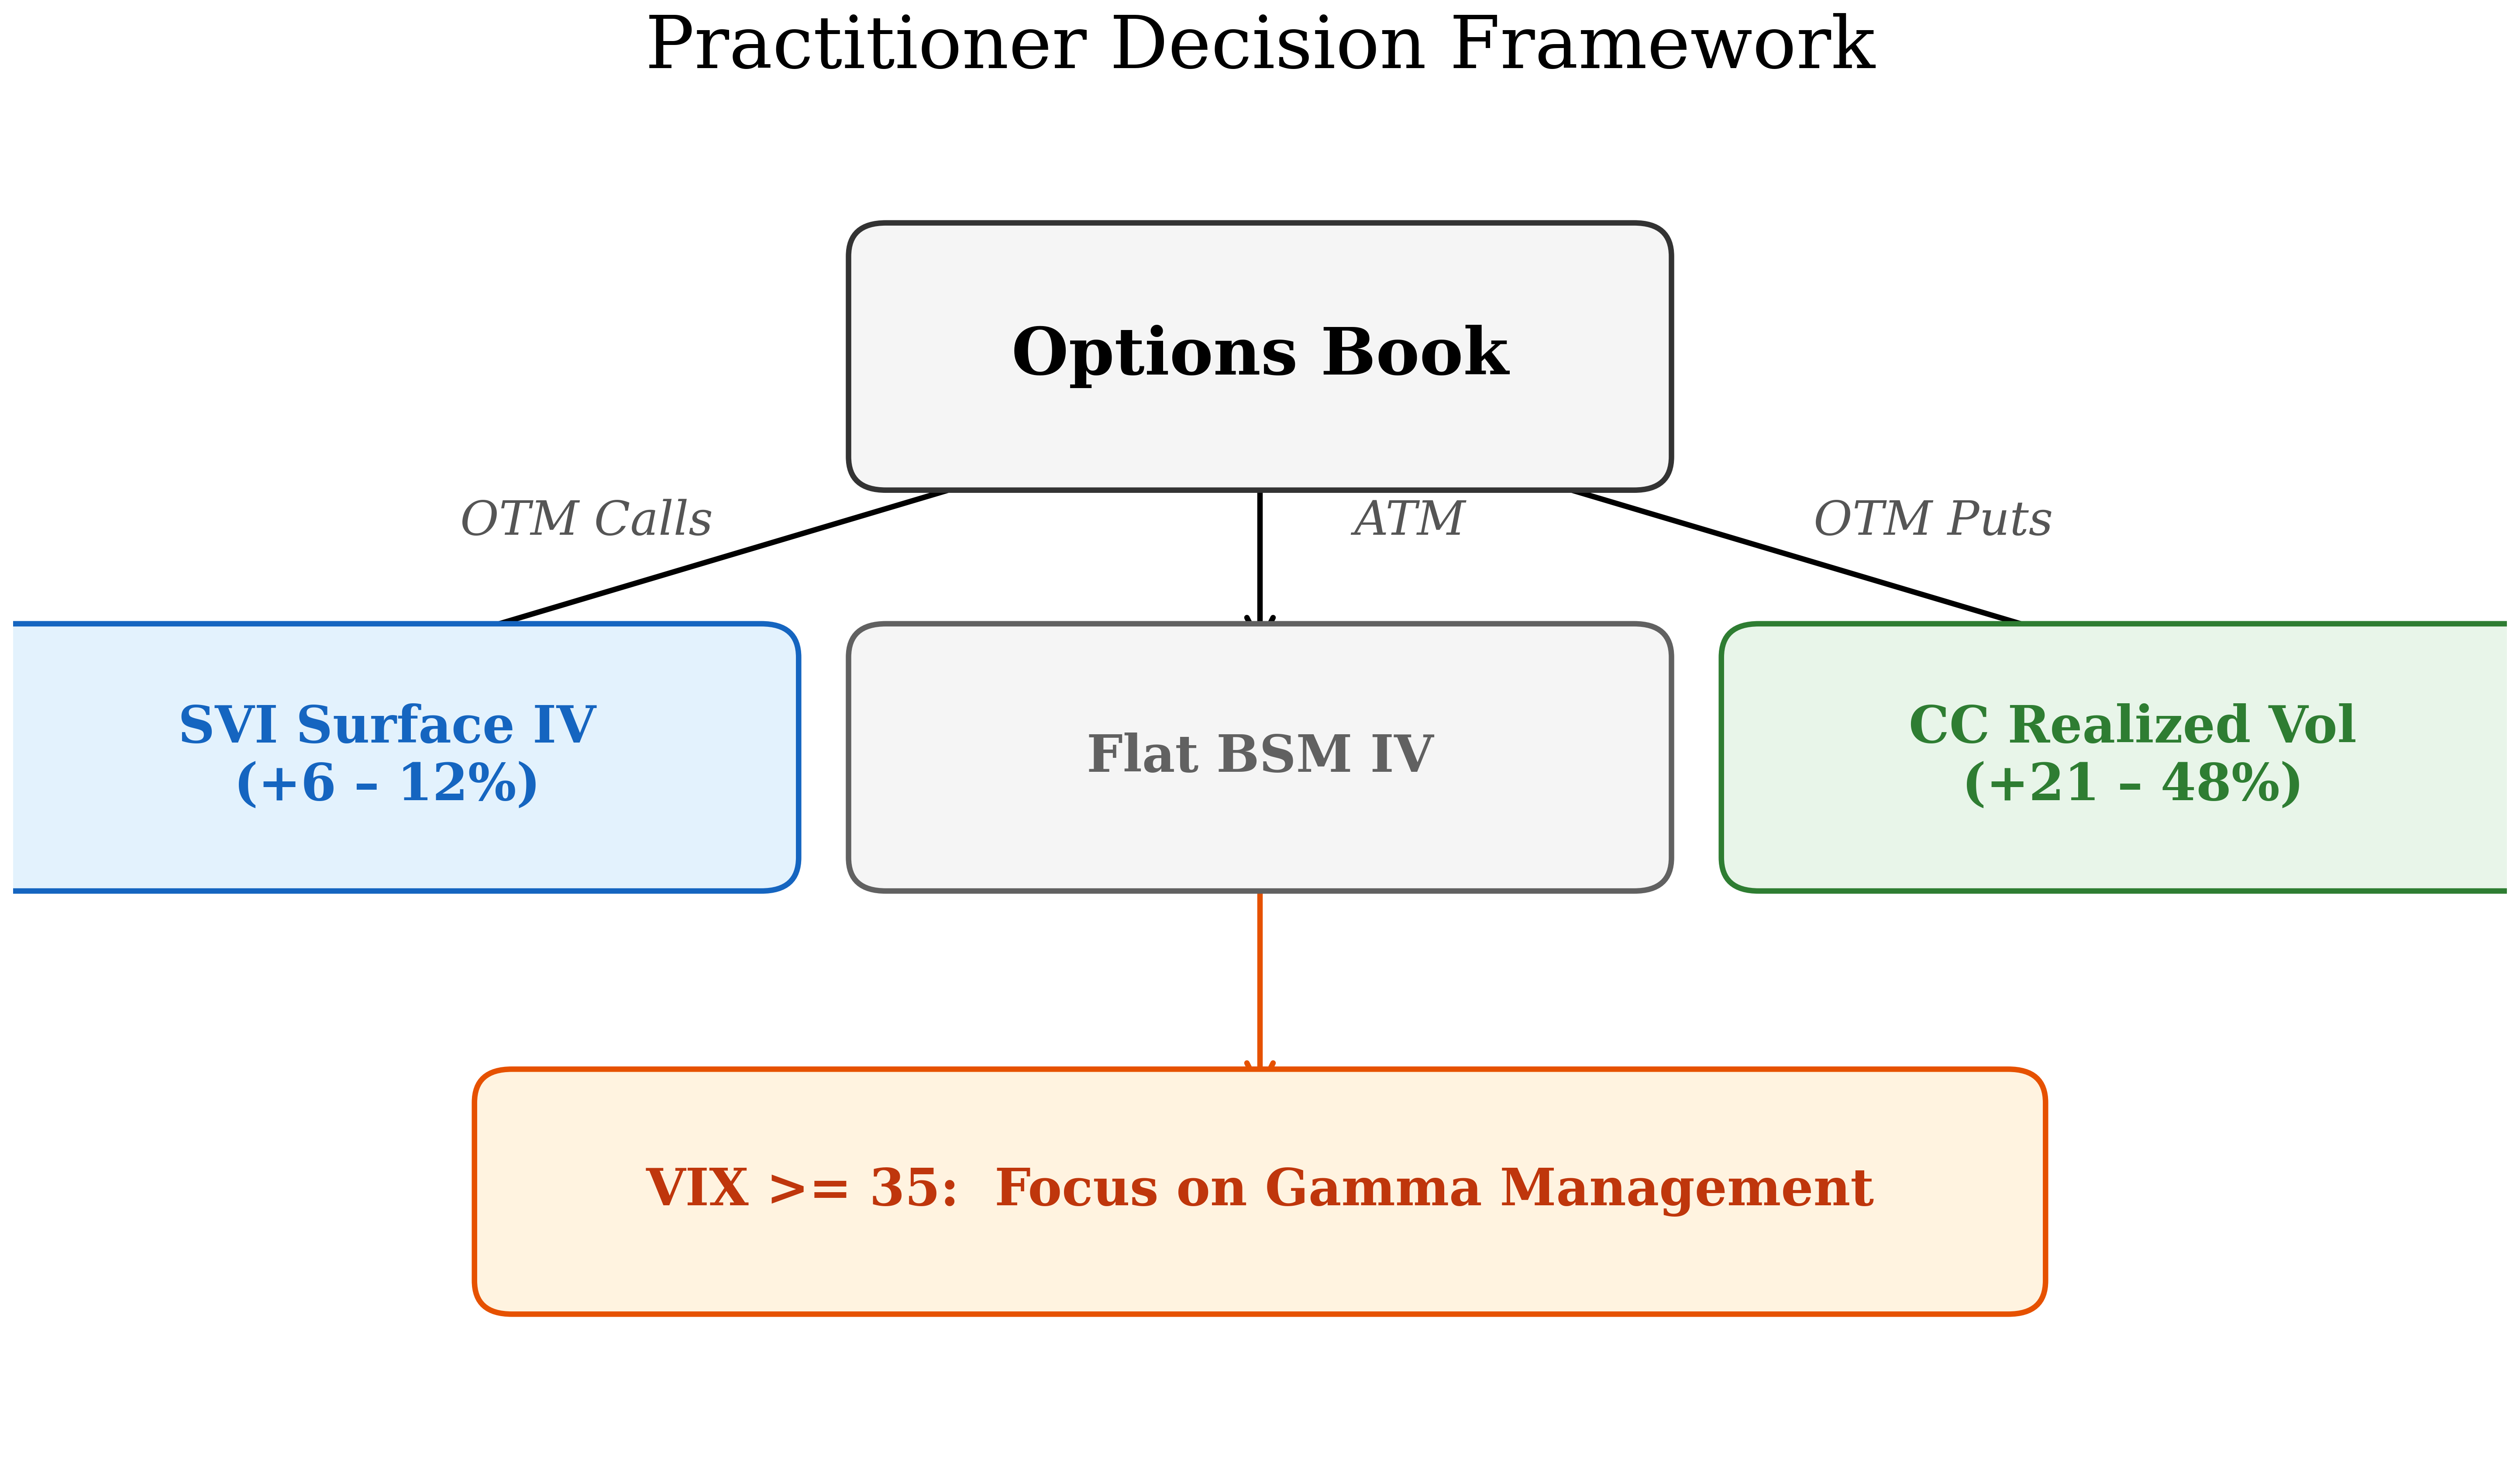
\includegraphics[width=0.85\textwidth]{fig_poster_flowchart.png}

\section*{DELTA-GAMMA HEDGING}
Complementing the empirical backtest, a 50{,}000-path Monte Carlo simulation validates the delta-gamma hedging extension:
\begin{center}
\begin{tabular}{lcc}
\hline
& \textbf{Delta-Only} & \textbf{Delta-Gamma} \\
\hline
P\&L Std (\$) & 0.44 & 0.24 \\
95\% Range & [$-$0.92, +0.90] & [$-$0.35, +0.32] \\
Std Reduction & --- & \textbf{46\%} \\
\hline
\end{tabular}
\end{center}
Neutralizing gamma directly eliminates the dominant source of hedging variance, consistent with the P\&L attribution finding that all three components scale with $\Gamma$.

\section*{ECONOMIC SIGNIFICANCE}
For a desk hedging \$1B notional in SPX options, a 5.8\% reduction in hedging error standard deviation translates to approximately 5--8\% lower Value-at-Risk, freeing risk capital for additional trading activity. The moneyness-conditional strategy---using SVI for OTM calls and CC RV for OTM puts---captures benefits across the entire option book.

\section*{TECHNICAL VALIDATION}
\begin{itemize}[nosep]
\item 80 unit tests spanning put-call parity, binomial convergence, variance reduction, Greek accuracy
\item Put-call parity validated to $< 10^{-10}$
\item Sub-basis-point cross-consistency across 3 pricing engines (BSM analytical, CRR binomial 1000-step, Monte Carlo 500k paths)
\item 8 analytical Greeks, finite-difference validation $<$ 0.1\% error
\item 3{,}069 SVI slices calibrated, 98\% convergence rate
\item Durrleman butterfly arbitrage checks: 68.6\% arb-free (82.4\% for RMSE $<$ 25 bps)
\item Delta-gamma hedging simulation: 46\% P\&L std reduction on 50{,}000 simulated paths
\end{itemize}

\section*{FUTURE WORK}
\begin{itemize}[nosep]
\item Extension to single-stock options (AAPL, NVDA) --- test American-style with earnings dynamics
\item Heston/SABR model comparison --- model-based deltas vs.\ BSM with alternative vol inputs
\item Deep hedging benchmark --- neural network comparison
\end{itemize}

\section*{CONTACT}
\begin{minipage}[c]{0.72\textwidth}
Zaid Annigeri | ma.zaid@rutgers.edu\\
GitHub: github.com/zaid282802/options-pricing-hedging\\
Full thesis and code available upon request\\
Future Alpha 2026 | March 31--April 1 | Brooklyn Marriott
\end{minipage}\hfill
\begin{minipage}[c]{0.22\textwidth}

\includegraphics[width=\linewidth]{qr_github.png}
\end{minipage}

\end{document}
